% Object relations and call hierarchy of the reseed / entropy polling
% mechanism of Botan's stateful RNGs (HMAC_DRBG), as of Botan 3.12.0.
%
% Source files depicted (Botan 3.12.0):
%   src/lib/rng/stateful_rng/stateful_rng.cpp  (reseed_check, reseed_from_*)
%   src/lib/rng/rng.cpp                        (base class reseed helpers)
%   src/lib/entropy/entropy_srcs.cpp           (Entropy_Sources::poll)
%
% Render with:  pdflatex rng_reseed.tex
%               pdftocairo -svg rng_reseed.pdf rng_reseed.svg
% (see figures/README.md)
\documentclass[tikz,border=8pt]{standalone}
\usepackage{tgheros}
\renewcommand{\familydefault}{\sfdefault}
\usetikzlibrary{positioning,arrows.meta,fit,calc}

\begin{document}
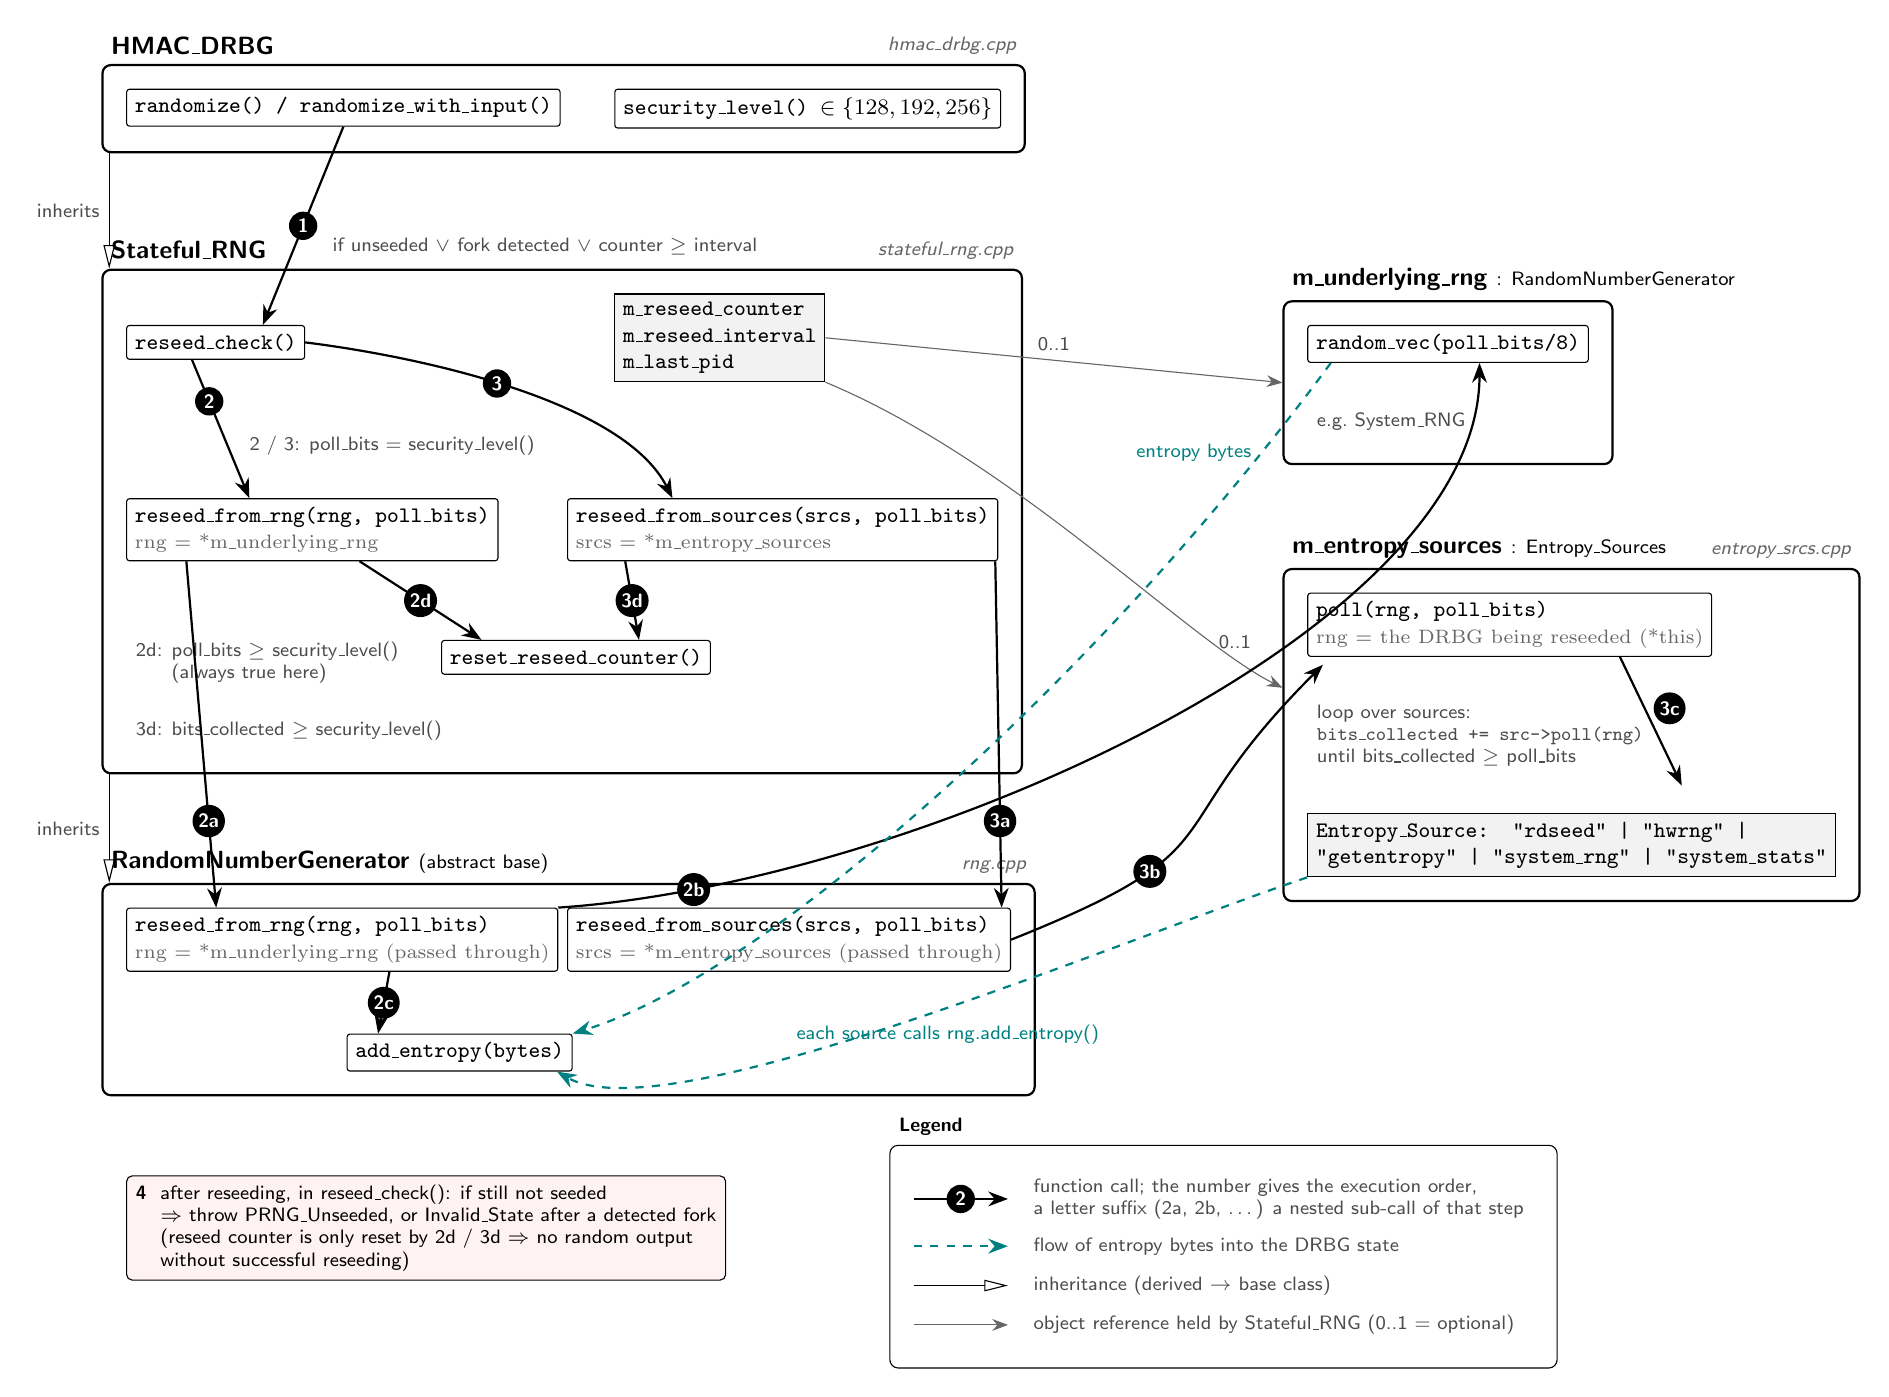
\begin{tikzpicture}[
    x=1mm, y=1mm,
    font=\small,
    method/.style={draw, rectangle, rounded corners=1pt, fill=white,
                   font=\ttfamily\footnotesize, inner sep=3pt, align=left,
                   anchor=north west},
    field/.style={draw, rectangle, fill=black!5,
                  font=\ttfamily\footnotesize, inner sep=3pt, align=left,
                  anchor=north west},
    classframe/.style={draw, thick, rounded corners=3pt, inner sep=3mm},
    classtitle/.style={font=\bfseries\small, anchor=south west},
    filelabel/.style={font=\itshape\scriptsize, anchor=south east, text=black!60},
    call/.style={-{Stealth[length=2.5mm]}, thick},
    entropy/.style={-{Stealth[length=2.5mm]}, thick, dashed, teal},
    inherit/.style={-{Triangle[open, length=3mm]}, thin},
    assoc/.style={-{Stealth[length=2mm]}, thin, black!60},
    num/.style={circle, fill=black, text=white, inner sep=1pt,
                font=\scriptsize\bfseries, minimum size=3.6mm},
    note/.style={font=\scriptsize, align=left, text=black!70},
  ]

  % ================================================================ HMAC_DRBG
  \node[method] (randomize) at (0,0) {randomize() / randomize\_with\_input()};
  \node[method] (seclevel) at (62,0) {security\_level() $\in\{128,192,256\}$};
  \node[classframe, fit=(randomize)(seclevel)] (hmacdrbg) {};
  \node[classtitle] at (hmacdrbg.north west) {HMAC\_DRBG};
  \node[filelabel]  at (hmacdrbg.north east) {hmac\_drbg.cpp};

  % ============================================================== Stateful_RNG
  \node[method] (reseedcheck)  at (0,-30)  {reseed\_check()};
  \node[field]  (state)        at (62,-26) {m\_reseed\_counter\\ m\_reseed\_interval\\ m\_last\_pid};
  \node[method] (srngfromrng)  at (0,-52)
      {reseed\_from\_rng(rng, poll\_bits)\\
       {\scriptsize\color{black!60}\rmfamily rng = *m\_underlying\_rng}};
  \node[method] (srngfromsrcs) at (56,-52)
      {reseed\_from\_sources(srcs, poll\_bits)\\
       {\scriptsize\color{black!60}\rmfamily srcs = *m\_entropy\_sources}};
  \node[method] (resetcounter) at (40,-70) {reset\_reseed\_counter()};
  \node[note, anchor=north west] (twodnote) at (0,-69)
      {2d: poll\_bits $\geq$ security\_level()\\
       \phantom{2d: }(always true here)};
  \node[note, anchor=north west] (threednote) at (0,-79)
      {3d: bits\_collected $\geq$ security\_level()};
  \node[classframe,
        fit=(reseedcheck)(state)(srngfromrng)(srngfromsrcs)(resetcounter)(twodnote)(threednote)]
      (statefulrng) {};
  \node[classtitle] at (statefulrng.north west) {Stateful\_RNG};
  \node[filelabel]  at (statefulrng.north east) {stateful\_rng.cpp};

  % ===================================================== RandomNumberGenerator
  \node[method] (basefromrng)  at (0,-104)
      {reseed\_from\_rng(rng, poll\_bits)\\
       {\scriptsize\color{black!60}\rmfamily rng = *m\_underlying\_rng (passed through)}};
  \node[method] (basefromsrcs) at (56,-104)
      {reseed\_from\_sources(srcs, poll\_bits)\\
       {\scriptsize\color{black!60}\rmfamily srcs = *m\_entropy\_sources (passed through)}};
  \node[method] (addentropy)   at (28,-120) {add\_entropy(bytes)};
  \node[classframe, fit=(basefromrng)(basefromsrcs)(addentropy)] (rngbase) {};
  \node[classtitle] at (rngbase.north west)
      {RandomNumberGenerator \normalfont\scriptsize(abstract base)};
  \node[filelabel]  at (rngbase.north east) {rng.cpp};

  % ============================================================ underlying RNG
  \node[method] (randomvec) at (150,-30) {random\_vec(poll\_bits/8)};
  \node[note, anchor=north west] (urngnote) at (150,-40) {e.g.\ System\_RNG};
  \node[classframe, fit=(randomvec)(urngnote)] (urng) {};
  \node[classtitle] at (urng.north west)
      {m\_underlying\_rng \normalfont\scriptsize: RandomNumberGenerator};

  % =========================================================== Entropy_Sources
  \node[method] (poll)     at (150,-64)
      {poll(rng, poll\_bits)\\
       {\scriptsize\color{black!60}\rmfamily rng = the DRBG being reseeded (*this)}};
  \node[note, anchor=north west] (pollnote) at (150,-77)
      {loop over sources:\\
       \ttfamily bits\_collected += src->poll(rng)\rmfamily\\
       until bits\_collected $\geq$ poll\_bits};
  \node[field]  (sources)  at (150,-92)
      {Entropy\_Source: "rdseed" | "hwrng" |\\
       "getentropy" | "system\_rng" | "system\_stats"};
  \node[classframe, fit=(poll)(pollnote)(sources)] (entsrcs) {};
  \node[classtitle] at (entsrcs.north west)
      {m\_entropy\_sources \normalfont\scriptsize: Entropy\_Sources};
  \node[filelabel]  at (entsrcs.north east) {entropy\_srcs.cpp};

  % ============================================================== inheritance
  \draw[inherit] ($(hmacdrbg.south west)+(1,0)$) -- ($(statefulrng.north west)+(1,0)$)
      node[midway, left, note] {inherits};
  \draw[inherit] ($(statefulrng.south west)+(1,0)$) -- ($(rngbase.north west)+(1,0)$)
      node[midway, left, note] {inherits};

  % ============================================================= associations
  \draw[assoc] (state.east) -- (urng.west)
      node[midway, above, note] {0..1};
  \draw[assoc] (state.south east) .. controls +(24,-10) and +(-12,6) ..
      ($(entsrcs.west)+(0,6)$)
      node[pos=0.85, above, note] {0..1};

  % ============================================================== call arrows
  % (1) randomize -> reseed_check
  \draw[call] (randomize.south) -- ($(reseedcheck.north)+(6,0)$)
      node[num, midway] {1};
  \node[note, anchor=west] at (25,-20)
      {if unseeded $\lor$ fork detected $\lor$ counter $\geq$ interval};

  % (2) reseed_check -> Stateful_RNG::reseed_from_rng
  \draw[call] ($(reseedcheck.south)+(-3,0)$) -- ($(srngfromrng.north)+(-8,0)$)
      node[num, pos=0.3] {2}
      node[note, pos=0.62, right=1.5mm] {2 / 3: poll\_bits = security\_level()};

  % (3) reseed_check -> Stateful_RNG::reseed_from_sources
  \draw[call] (reseedcheck.east) .. controls +(16,-2) and +(-6,12) ..
      ($(srngfromsrcs.north)+(-14,0)$)
      node[num, pos=0.45] {3};

  % (2d) reset counter (condition always true on this path)
  \draw[call] ($(srngfromrng.south)+(6,0)$) -- ($(resetcounter.north)+(-12,0)$)
      node[num, pos=0.5] {2d};

  % (3d) reset counter if enough collected
  \draw[call] ($(srngfromsrcs.south)+(-20,0)$) -- ($(resetcounter.north)+(8,0)$)
      node[num, pos=0.5] {3d};

  % (2a) override -> base
  \draw[call] ($(srngfromrng.south)+(-16,0)$) -- ($(basefromrng.north)+(-16,0)$)
      node[num, pos=0.75] {2a};

  % (3a) override -> base
  \draw[call] ($(srngfromsrcs.south)+(27,0)$) -- ($(basefromsrcs.north)+(27,0)$)
      node[num, pos=0.75] {3a};

  % (2b) base reseed_from_rng -> underlying RNG random_vec
  \draw[call] (basefromrng.north east) .. controls +(45,3) and +(0,-34) ..
      ($(randomvec.south)+(4,0)$)
      node[num, pos=0.12] {2b};

  % (2c) base reseed_from_rng -> add_entropy
  \draw[call] ($(basefromrng.south)+(6,0)$) -- ($(addentropy.north west)+(4,0)$)
      node[num, pos=0.5] {2c};

  % (3b) base reseed_from_sources -> Entropy_Sources::poll
  \draw[call] (basefromsrcs.east) .. controls +(30,12) and +(-22,-22) ..
      ($(poll.south west)+(2,-1)$)
      node[num, pos=0.3] {3b};

  % (3c) poll -> each source poll
  \draw[call] ($(poll.south)+(14,0)$) -- ($(sources.north)+(14,3.5)$)
      node[num, pos=0.4, right=1mm] {3c};

  % ========================================================= entropy data flow
  \draw[entropy] ($(randomvec.south west)+(3,0)$) .. controls +(-28,-38) and +(26,8) ..
      (addentropy.north east)
      node[pos=0.1, left, note, teal] {entropy bytes};
  \draw[entropy] (sources.south west) .. controls +(-24,-8) and +(14,-8) ..
      ($(addentropy.south east)+(-2,0)$)
      node[pos=0.45, below=1mm, note, teal, align=center]
        {each source calls rng.add\_entropy()};

  % ============================================================== failure note
  \node[draw, rounded corners=2pt, fill=red!5, note, text=black,
        anchor=north west] (fail) at (0,-138)
      {\textbf{4} \ after reseeding, in reseed\_check(): if still not seeded\\
       \phantom{\textbf{4} \ }$\Rightarrow$ throw PRNG\_Unseeded, or Invalid\_State after a detected fork\\
       \phantom{\textbf{4} \ }(reseed counter is only reset by 2d / 3d $\Rightarrow$ no random output\\
       \phantom{\textbf{4} \ }without successful reseeding)};

  % ==================================================================== legend
  \coordinate (leg1) at (100,-141);
  \coordinate (leg2) at (100,-147);
  \coordinate (leg3) at (100,-152);
  \coordinate (leg4) at (100,-157);
  \draw[call] (leg1) -- +(12,0);
  \node[num] at ($(leg1)+(6,0)$) {2};
  \node[note, anchor=west] (legl1) at ($(leg1)+(14,0)$)
      {function call; the number gives the execution order,\\
       a letter suffix (2a, 2b, \dots) a nested sub-call of that step};
  \draw[entropy] (leg2) -- +(12,0);
  \node[note, anchor=west] (legl2) at ($(leg2)+(14,0)$)
      {flow of entropy bytes into the DRBG state};
  \draw[inherit] (leg3) -- +(12,0);
  \node[note, anchor=west] (legl3) at ($(leg3)+(14,0)$)
      {inheritance (derived $\rightarrow$ base class)};
  \draw[assoc] (leg4) -- +(12,0);
  \node[note, anchor=west] (legl4) at ($(leg4)+(14,0)$)
      {object reference held by Stateful\_RNG (0..1 = optional)};
  \node[classframe, thin, fit=(leg1)(leg4)(legl1)(legl2)(legl3)(legl4)] (legend) {};
  \node[classtitle, font=\bfseries\scriptsize] at (legend.north west) {Legend};

\end{tikzpicture}
\end{document}
